\section{Surface Heat Balances With Moveable Insulation}\label{surface-heat-balances-with-moveable-insulation}

In EnergyPlus, moveable insulation can be present either on the interior or exterior side of a particular construction. Different heat balances are impacted depending on the location of the moveable insulation.  Having moveable insulation on the interior side results in a modified form of the inside surface heat balance equation.  Having moveable insulation on the exterior side results in different cases for the outside surface heat balance.  Information on the modeling equations for each of these types of moveable insulation are shown in the next several sections.

\subsection{Inside Heat Balance with Interior Moveable Insulation}\label{inside-heat-balance-with-interior-moveable-insulation}

There are two different heat balances which must be maintained to model interior moveable insulation.  At both the interface between the zone air and the moveable insulation and the interface between the moveable insulation and the surface (wall, roof, etc.), the following general heat balance must be maintained:

\begin{equation}
Conductive + Convective + Radiative = 0
\label{eq:BasicSteadyStateHeatBalanceEquation}
\end{equation}

One significant complication of the inside heat balance is the fact that surfaces within the same zone can interact with each other radiatively.  This means that a solution for all surface temperatures must be done at the same time to maintain a radiation heat balance among the surfaces.  This requires some iteration of the inside surface heat balance as will be seen in the equations that are shown later in this subsection.

Another complication of the inside heat balance relates to the presense of moveable insulation.  When moveable insulation is present, a second heat balance equation is required to determine the temperature at both the air-moveable insulation interface as well as the moveable insulation-surface interface.  This sets up a system of two equations with two unknowns: the temperatures at the air-moveable insulation interface and the moveable insulation-surface interface.

Applying the basic steady state heat balance equation at each of these interfaces results in the following two equations:

\begin{equation}
H_c \cdot \left( T_a - T_{mi} \right) + Q_{lw} + H_{mi} \cdot  \left( T_i - T_{mi} \right) + I_t \cdot  \left( T_{old} - T_{mi} \right) = 0
\label{eq:InsideHBAirMovInsInterface}
\end{equation}

\begin{equation}
H_{mi} \cdot \left( T_{mi} - T_i \right) + Q_{sw} + Q_{cond} = 0
\label{eq:InsideHBMovInsSurfInterface}
\end{equation}

where:

\(H_c\) is the convective heat transfer coefficient between the moveable insulation and the air

\(T_a\) is the zone air temperature

\(T_{mi}\) is the temperature at the interface between the air and the moveable insulation

\(Q_{lw}\) is the long wavelength radiation incident on the interface between the air and the moveable insulation

\(H_{mi}\) is the U-value of the moveable insulation material

\(T_i\) is the temperature at the interface between the moveable insulation and the surface

\(I_t\) is a damping constant for iterating to achieve a stable radiant exchange between zone surfaces

\(T_{old}\) is the previous surface temperature at the last solution iteration

\(Q_{sw}\) is the short wavelength radiation incident on the interface between the moveable insulation and the surface

\(Q_{cond}\) is the conduction heat transfer through the surface.

Equation~\ref{eq:InsideHBAirMovInsInterface} is the heat balance at the air-moveable insulation interface and can be rearranged to solve for the temperature at this interface, T\(_{mi}\).  Equation~\ref{eq:InsideHBMovInsSurfInterface} is the heat balance at the moveable insulation-surface interface and provides a second equation for T\(_{mi}\).  Both equations leave T\(_{mi}\) as a function of T\(_{i}\) and other known quantities as shown below.

It should be noted that there are some assumptions built into these equations.  First, all long wavelength radiation whether from other surfaces or other elements (such as heat sources which add radiation to the zone) is all assumed to be incident at and influence the air-moveable insulation interface.  This also means that no long wavelength radiation is transmitted through the moveable insulation to the moveable insulation-surface interface.  Second, all short wavelength radiation is assumed to be transmitted through the moveable insulation to the moveable-insulation interface.  This is a simplification that is consistent with transparent insulation and assumes that the moveable insulation material itself does not absorb any short wavelength as it passes through it.  Third, the term Q\(_{cond}\) includes several terms that all relate to the method for calculating heat conduction through the actual surface to which the moveable insulation is attached.  Finally, the moveable insulation material is sufficiently lightweight thermally that it has no thermal mass and it can be treated as an equivalent resistance.

Equation~\ref{eq:InsideHBAirMovInsInterface} can be rearranged to obtain:

\begin{equation}
\left( H_c + H_{mi} + I_t \right) \cdot T_m = H_c \cdot T_a + H_m \cdot T_i + Q_{lw} + I_t \cdot T_{old}
\label{eq:RearrangedHBAirMovIns}
\end{equation}

When Equation~\ref{eq:InsideHBMovInsSurfInterface} is rearranged to solve for \(T_m\) and this is substituted back into Equation~\ref{eq:RearrangedHBAirMovIns}, one obtains a single equation that allows for the solution of \(T_i\).  This can then be used to solve for \(T_{mi}\).

The C++ code that is used to solve for \(T_i\) and \(T_{mi}\) for cases where moveable insulation is present on the interior side is shown below.

\begin{lstlisting}
F1 = HMovInsul / (HMovInsul + HConvIn_surf + IterDampConst);

SurfTempIn(SurfNum) = (SurfCTFConstInPart(SurfNum) + SurfOpaqQRadSWInAbs(SurfNum) + construct.CTFCross(0) * TH11 +
                       F1 * (SurfQRadThermInAbs(SurfNum) + HConvIn_surf * RefAirTemp(SurfNum) +
                       SurfNetLWRadToSurf(SurfNum) + SurfQdotRadHVACInPerArea(SurfNum) +
                       QAdditionalHeatSourceInside(SurfNum) +
                       IterDampConst * SurfTempInsOld(SurfNum)))
                       / (construct.CTFInside(0) + HMovInsul - F1 * HMovInsul); 

SurfTempInTmp(SurfNum) = (construct.CTFInside(0) * SurfTempIn(SurfNum) +
                          HMovInsul * SurfTempIn(SurfNum) -
                          SurfOpaqQRadSWInAbs(SurfNum) - SurfCTFConstInPart(SurfNum) -
                          construct.CTFCross(0) * TH11) / (HMovInsul);
\end{lstlisting}

\subsection{Outside Heat Balance Cases for Exterior Moveable Insulation}\label{outside-heat-balance-cases-for-exterior-moveable-insulation}

Just like at the inside surface-air interface, a heat balance must exist at the outside surface-air interface. The incoming conductive, convective, and radiative fluxes must sum up to zero as shown in Equation~\ref{eq:BasicSteadyStateHeatBalanceEquation}.

In contrast to the internal surface heat balance that treats all surfaces simultaneously, the external thermal balance for each surface is performed independent of all other surfaces. This implies that there is no direct interaction between the individual surfaces.

TARP includes four possible representations for the basic outside surface heat balance. The first two depend on which of the optimal surface conductance algorithms the user selects. The simple outside surface conductance that includes both the convective and thermal interchange between the surface and the environment in a single coefficient, is represented by the thermal network in Figure~\ref{fig:thermal-network-for-simple-outside-surface}. Equation~\ref{eq:BasicSteadyStateHeatBalanceEquation} can also be expressed as:

\begin{equation}
\left[ {{\rm{KO}}{{\rm{P}}_{\rm{t}}} + {{\rm{Y}}_{\rm{0}}}\cdot {\rm{T}}{{\rm{I}}_t} - {{\rm{X}}_{\rm{0}}}\cdot {\rm{T}}{{\rm{O}}_{\rm{t}}}} \right]{\rm{ + }}\left[ {{\rm{HO}}\cdot \left( {{{\rm{T}}_{\rm{a}}} - {\rm{T}}{{\rm{O}}_t}} \right)} \right]{\rm{  + QSO  =  0}}
\end{equation}

This can be solved for the outside surface temperature.

\begin{equation}
{\rm{T}}{{\rm{O}}_{\rm{t}}}{\rm{ = }}\left[ {\frac{{{\rm{KO}}{{\rm{P}}_{\rm{t}}} + {\rm{QSO}} + {{\rm{Y}}_0}\cdot {\rm{T}}{{\rm{I}}_{\rm{t}}}{\rm{ + HO}}\cdot {{\rm{T}}_{\rm{a}}}}}{{{{\rm{X}}_{\rm{0}}}{\rm{ + HO}}}}} \right]{\rm{  }}
\label{eq:OutsideSurfTempHeatBalEq}
\end{equation}

The detailed outside surface conductance model considers convection and radiant interchange with the sky and with the ground as separate factors. Its use in the outside thermal balance is shown in Figure~\ref{fig:thermal-network-for-detailed-outside-surface}. In this case, Equation~\ref{eq:BasicSteadyStateHeatBalanceEquation} can be expanded to give:

\begin{equation}
\left[ {{\rm{KO}}{{\rm{P}}_{\rm{t}}}{\rm{ + }}{{\rm{Y}}_{\rm{0}}}\cdot {\rm{T}}{{\rm{I}}_{\rm{t}}}{\rm{ - }}{{\rm{X}}_{\rm{0}}}\cdot {\rm{T}}{{\rm{O}}_{\rm{t}}}} \right]{\rm{ + }}\left[ {{\rm{HA}}\cdot \left( {{{\rm{T}}_{\rm{a}}}{\rm{ - T}}{{\rm{O}}_{\rm{t}}}} \right){\rm{ + HS}}\cdot \left( {{{\rm{T}}_{\rm{s}}}{\rm{ - T}}{{\rm{O}}_{\rm{t}}}} \right){\rm{ + HG}}\cdot \left( {{{\rm{T}}_{\rm{g}}}{\rm{ - T}}{{\rm{O}}_{\rm{t}}}} \right)} \right]{\rm{  + QSO  =  0  }}
\label{eq:MoreDetailedOutsideSurfHeatBalEq}
\end{equation}

This can be solved for the outside surface temperature:

\begin{equation}
{\rm{T}}{{\rm{O}}_{\rm{t}}}{\rm{ = }}\left[ {\frac{{{\rm{KO}}{{\rm{P}}_{\rm{t}}} + {\rm{QSO}} + {{\rm{Y}}_0}\cdot {\rm{T}}{{\rm{I}}_{\rm{t}}}{\rm{ + HA}}\cdot {{\rm{T}}_{\rm{a}}}{\rm{ + HS}}\cdot {{\rm{T}}_{\rm{s}}}{\rm{ + HG}}\cdot {{\rm{T}}_{\rm{g}}}}}{{{{\rm{X}}_{\rm{0}}}{\rm{ + HA + HS + HG}}}}} \right]{\rm{  }}
\end{equation}

The third and fourth representations occur when the outside surface has been covered with movable insulation. The insulation has a conductance of UM. The thermal network in Figure~\ref{fig:thermal-network-for-outside-moveable} represents this case.The insulation must be mass-less because it is not generally possible to perform a correct thermal balance at the juncture of two surfaces each modeled by CTF.

The equation for the thermal balance between the surface and the insulation is:

\begin{equation}
\left[ {{\rm{KO}}{{\rm{P}}_{\rm{t}}} + {{\rm{Y}}_{\rm{0}}}\cdot {\rm{T}}{{\rm{I}}_t} - {{\rm{X}}_{\rm{0}}}\cdot {\rm{T}}{{\rm{O}}_{\rm{t}}} + {\rm{UM}}\cdot \left( {{\rm{TM - T}}{{\rm{O}}_{\rm{t}}}} \right)} \right]{\rm{ + QSO  =  0}}
\end{equation}

Which can be rewritten to solve for TO:

\begin{equation}
{\rm{T}}{{\rm{O}}_{\rm{t}}}{\rm{ = }}\left[ {\frac{{{\rm{KO}}{{\rm{P}}_{\rm{t}}} + {\rm{QSO}} + {{\rm{Y}}_0}\cdot {\rm{T}}{{\rm{I}}_{\rm{t}}}{\rm{ + UM}}\cdot {\rm{TM}}}}{{{{\rm{X}}_{\rm{0}}}{\rm{ + UM}}}}} \right]{\rm{  }}
\label{eq:HeatBalEqforTo}
\end{equation}

Depending on whether or not the detailed or simple algorithm for surface conductance is being used, there are two expressions for TM, the outside temperature of the insulation. For the simple conductance:

\begin{equation}
{\rm{TM}} = \left[ {\frac{{{\rm{QSM + UM}}\cdot {\rm{T}}{{\rm{O}}_{\rm{t}}}{\rm{ + HO}}\cdot {{\rm{T}}_{\rm{a}}}}}{{{\rm{UM + HO}}}}} \right]
\label{eq:OutTempMovableInsulation}
\end{equation}

For the detailed conductance:

\begin{equation}
{\rm{T}}{{\rm{O}}_{\rm{t}}}{\rm{ = }}\left[ {\frac{{{\rm{QSM}} + {\rm{UM}}\cdot {\rm{T}}{{\rm{O}}_{\rm{t}}}{\rm{ + HA}}\cdot {{\rm{T}}_{\rm{a}}}{\rm{ + HS}}\cdot {{\rm{T}}_{\rm{s}}}{\rm{ + HG}}\cdot {{\rm{T}}_{\rm{g}}}}}{{{\rm{UM + HA + HS + HG}}}}} \right]{\rm{  }}
\label{eq:TOtEquationDetailedConductance}
\end{equation}

In this case the values of HA, HS and HG must be found by using an estimated value of TM in place of TO.

\begin{figure}[hbtp] % fig 29
\centering
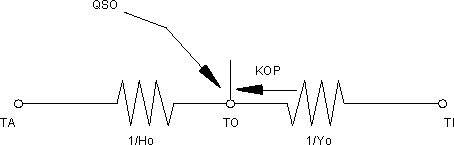
\includegraphics[width=0.9\textwidth, height=0.9\textheight, keepaspectratio=true]{media/image420.png}
\caption{Thermal Network for Simple Outside Surface Coefficient \protect \label{fig:thermal-network-for-simple-outside-surface}}
\end{figure}

\begin{figure}[hbtp] % fig 30
\centering
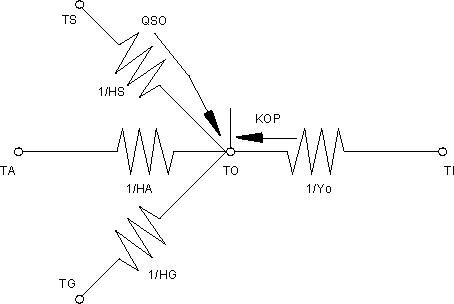
\includegraphics[width=0.9\textwidth, height=0.9\textheight, keepaspectratio=true]{media/image421.png}
\caption{Thermal Network for Detailed Outside Surface Coefficient \protect \label{fig:thermal-network-for-detailed-outside-surface}}
\end{figure}

\begin{figure}[hbtp] % fig 31
\centering
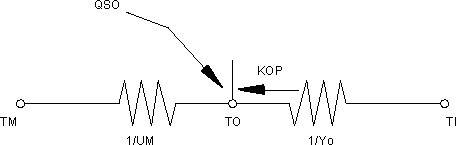
\includegraphics[width=0.9\textwidth, height=0.9\textheight, keepaspectratio=true]{media/image422.png}
\caption{Thermal Network for Outside Moveable Insulation \protect \label{fig:thermal-network-for-outside-moveable}}
\end{figure}

\subsection{Heat Balance Cases}\label{heat-balance-cases}

TO\(_{t}\) and TI\(_{t}\) are related through the Y\(_{0}\)CTF. However TI\(_{t}\) is also unknown. While it is possible to combine the outside and the inside surface heat balances to compute TO\(_{t}\) and TI\(_{t}\) simultaneously, TARP uses a simpler procedure where TO\(_{t}\) is based on a previous value of TI. When Y\(_{0}\) is small, as occurs in well insulated or very massive surfaces, TI\(_{t}\) can be replaced by TI\(_{t-1}\) (which is known for the previous hour's heat balance) without significantly effecting the value of TO\(_{t}\) When Y\(_{0}\) is large, TO and TI can so strongly be coupled that separate outside and inside heat balances do not work because the environment and zone temperatures have negligible influence on the heat balances. The TARP uses the inside surface heat balance to couple TO\(_{t}\) with TZ and TR. These two temperatures are less strongly influenced by TO and allow a reasonable heat balance. On the first heat balance iteration, TZ and TR are the values at time t-1. The user may optionally require that TO\(_{t}\) be recomputed with every iteration of TI\(_{t}\). ~In this case TZ and TR have values from the previous iteration and a true simultaneous solution is achieved. In most conventional constructions, recomputing TO\(_{t}\) does not significantly change the computed zone loads and temperatures. The inside surface heat balance is given by:

\begin{equation}
{\rm{T}}{{\rm{I}}_{\rm{t}}} = \left[ {\frac{{KI{P_t} + QSI + HC\cdot TZ + HR\cdot TR + {Y_0}\cdot TO}}{{{Z_0} + HC + HR}}} \right]
\label{eq:InsideSurfTempHeatBalEq}
\end{equation}

The surface heat balances can be combined in eight ways according to conditions for calculations of the outside surface temperature:

\begin{equation}
{F_1} = \left[ {\frac{{{Y_0}}}{{{Z_0} + HI + HR}}} \right]
\end{equation}

\begin{equation}
{F_2} = \left[ {\frac{{UM}}{{UM + HO}}} \right]
\end{equation}

\begin{equation}
{F_3} = \left[ {\frac{{UM}}{{UM + HA + HS + HG}}} \right]
\end{equation}

\subsubsection{Case1: Y\(_{0}\)~ small, simple conductance, no movable insulation:}\label{case1-yux5f0-small-simple-conductance-no-movable-insulation}

From Equation~\ref{eq:OutsideSurfTempHeatBalEq},

\begin{equation}
{\rm{T}}{{\rm{O}}_{\rm{t}}}{\rm{ = }}\left[ {\frac{{{\rm{KO}}{{\rm{P}}_{\rm{t}}} + {\rm{QSO}} + {{\rm{Y}}_0}\cdot {\rm{T}}{{\rm{I}}_{{\rm{t - 1}}}}{\rm{ + HO}}\cdot {{\rm{T}}_{\rm{a}}}}}{{{{\rm{X}}_{\rm{0}}}{\rm{ + HO}}}}} \right]{\rm{  }}
\end{equation}

\subsubsection{Case2: Y\(_{0}\) not small, simple conductance, no movable insulation:}\label{case2-yux5f0-not-small-simple-conductance-no-movable-insulation}

From Equations~\ref{eq:OutsideSurfTempHeatBalEq} and~\ref{eq:InsideSurfTempHeatBalEq}:

\begin{equation}
{\rm{T}}{{\rm{O}}_{\rm{t}}}{\rm{ = }}\left[ {\frac{{{\rm{KO}}{{\rm{P}}_{\rm{t}}} + {\rm{QSO}} + {\rm{HO}}\cdot {{\rm{T}}_{\rm{a}}} + {{\rm{F}}_1}\cdot \left( {{\rm{KI}}{{\rm{P}}_{\rm{t}}}{\rm{ + QSI + HI}}\cdot {\rm{TZ + HR}}\cdot {\rm{TR}}} \right)}}{{{{\rm{X}}_{\rm{0}}}{\rm{ + HO - }}{{\rm{F}}_{\rm{1}}}\cdot {{\rm{Y}}_0}}}} \right]{\rm{  }}
\end{equation}

\subsubsection{Case3: Y\(_{0}\)~ small, detailed conductance, no movable insulation:}\label{case3-yux5f0-small-detailed-conductance-no-movable-insulation}

From Equation~\ref{eq:MoreDetailedOutsideSurfHeatBalEq}:

\begin{equation}
{\rm{T}}{{\rm{O}}_{\rm{t}}}{\rm{ = }}\left[ {\frac{{{\rm{KO}}{{\rm{P}}_{\rm{t}}} + {\rm{QSO}} + {{\rm{Y}}_0}\cdot {\rm{T}}{{\rm{I}}_{{\rm{t - 1}}}}{\rm{ + HA}}\cdot {{\rm{T}}_{\rm{a}}} + {\rm{HS}}\cdot {{\rm{T}}_{\rm{s}}} + {\rm{HG}}\cdot {{\rm{T}}_{\rm{g}}}}}{{{{\rm{X}}_{\rm{0}}}{\rm{ + HA + HS + HG}}}}} \right]{\rm{  }}
\end{equation}

\subsubsection{Case4: Y\(_{0}\) not small, detailed conductance, no movable insulation:}\label{case4-yux5f0-not-small-detailed-conductance-no-movable-insulation}

From Equations~\ref{eq:MoreDetailedOutsideSurfHeatBalEq} and~\ref{eq:InsideSurfTempHeatBalEq}:

\begin{equation}
{\rm{T}}{{\rm{O}}_{\rm{t}}}{\rm{ = }}\left[ {\frac{{{\rm{KO}}{{\rm{P}}_{\rm{t}}} + {\rm{QSO}} + {\rm{HA}}\cdot {{\rm{T}}_{\rm{a}}} + {\rm{HS}}\cdot {{\rm{T}}_{\rm{s}}} + {\rm{HG}}\cdot {{\rm{T}}_{\rm{g}}} + {{\rm{F}}_{\rm{1}}}\cdot \left( {{\rm{KI}}{{\rm{P}}_{\rm{t}}}{\rm{ + QSI + HI}}\cdot {\rm{TZ + HR}}\cdot {\rm{TR}}} \right)}}{{{{\rm{X}}_{\rm{0}}}{\rm{ + HA + HS + HG - }}{{\rm{F}}_1}\cdot {{\rm{Y}}_0}}}} \right]{\rm{  }}
\end{equation}

\subsubsection{Case5: Y\(_{0}\)~ small, simple conductance, with movable insulation:}\label{case5-yux5f0-small-simple-conductance-with-movable-insulation}

From Equations~\ref{eq:HeatBalEqforTo} and~\ref{eq:OutTempMovableInsulation}:

\begin{equation}
TO_t = \left[ \frac{ KOP_t + QSO + Y_0 \cdot {TI_{t-1}} + F_2 \cdot \left( QSM + HO \cdot TM \right) } { X_0 + UM - F_2 \cdot UM } \right]
\label{eq:HeatBalanceEquationCase5}
\end{equation}

\subsubsection{Case6: Y\(_{0}\) not small, simple conductance, with movable insulation:}\label{case6-yux5f0-not-small-simple-conductance-with-movable-insulation}

From Equations~\ref{eq:HeatBalEqforTo}, ~\ref{eq:OutTempMovableInsulation} and~\ref{eq:InsideSurfTempHeatBalEq}:

\begin{equation}
{\rm{T}}{{\rm{O}}_{\rm{t}}}{\rm{ = }}\left[ {\frac{{{\rm{KO}}{{\rm{P}}_{\rm{t}}} + {\rm{QSO}} + {{\rm{F}}_2}\cdot \left( {{\rm{QSM + HO}}\cdot {{\rm{T}}_{\rm{a}}}} \right) + {{\rm{F}}_1}\cdot \left( {{\rm{KI}}{{\rm{P}}_{\rm{t}}}{\rm{ + QSI + HI}}\cdot {\rm{TZ + HR}}\cdot {\rm{TR}}} \right)}}{{{{\rm{X}}_{\rm{0}}} + {\rm{UM - }}{{\rm{F}}_{\rm{2}}}\cdot {\rm{UM - }}{{\rm{F}}_{\rm{1}}}\cdot {{\rm{Y}}_{\rm{0}}}}}} \right]{\rm{  }}
\label{eq:HeatBalanceEquationCase6}
\end{equation}

\subsubsection{Case7: Y\(_{0}\)~ small, detailed conductance, with movable insulation:}\label{case7-yux5f0-small-detailed-conductance-with-movable-insulation}

From Equations~\ref{eq:HeatBalEqforTo} and~\ref{eq:TOtEquationDetailedConductance}:

\begin{equation}
{\rm{T}}{{\rm{O}}_{\rm{t}}}{\rm{ = }}\left[ {\frac{{{\rm{KO}}{{\rm{P}}_{\rm{t}}} + {\rm{QSO}} + {{\rm{Y}}_0}\cdot {\rm{T}}{{\rm{I}}_{{\rm{t - 1}}}}{\rm{ + }}{{\rm{F}}_{\rm{3}}}\left( {{\rm{QSM + HA}}\cdot {{\rm{T}}_{\rm{a}}}{\rm{ + HS}}\cdot {{\rm{T}}_{\rm{s}}}{\rm{ + HG}}\cdot {{\rm{T}}_{\rm{g}}}} \right)}}{{{{\rm{X}}_{\rm{0}}}{\rm{ + UM - }}{{\rm{F}}_{\rm{3}}}\cdot {\rm{UM}}}}} \right]{\rm{  }}
\label{eq:HeatBalanceEquationCase7}
\end{equation}

\subsubsection{Case8: Y\(_{0}\) not small, detailed conductance, with movable insulation:}\label{case8-yux5f0-not-small-detailed-conductance-with-movable-insulation}

From Equations~\ref{eq:HeatBalEqforTo}, ~\ref{eq:TOtEquationDetailedConductance} and~\ref{eq:InsideSurfTempHeatBalEq}:

\begin{equation}
\medmuskip=0mu
\thinmuskip=0mu
\thickmuskip=0mu
\nulldelimiterspace=0pt
\scriptspace=0pt
{\rm{T}}{{\rm{O}}_{\rm{t}}}{\rm{ = }}\left[ {\frac{{{\rm{KO}}{{\rm{P}}_{\rm{t}}} + {\rm{QSO}} + {{\rm{F}}_1}\cdot \left( {{\rm{KI}}{{\rm{P}}_{\rm{t}}}{\rm{ + QSI + HI}}\cdot {\rm{TZ + HR}}\cdot {\rm{TR}}} \right){\rm{ + }}{{\rm{F}}_{\rm{3}}}\left( {{\rm{QSM + HA}}\cdot {{\rm{T}}_{\rm{a}}}{\rm{ + HS}}\cdot {{\rm{T}}_{\rm{s}}}{\rm{ + HG}}\cdot {{\rm{T}}_{\rm{g}}}} \right)}}{{{{\rm{X}}_{\rm{0}}}{\rm{ + UM - }}{{\rm{F}}_{\rm{3}}}\cdot {\rm{UM - }}{{\rm{F}}_{\rm{1}}}\cdot {{\rm{Y}}_{\rm{0}}}}}} \right]{\rm{  }}
\label{eq:HeatBalanceEquationCase8}
\end{equation}

\subsection{C++ Algorithm Examples}\label{c++-algorithm-examples}

These C++ code snippets show the implementation of these different cases.

\subsubsection{Case5: Y\(_{0}\)~ small, simple conductance, with movable insulation:}\label{case5-yux5f0-small-simple-conductance-with-movable-insulation-1}

From Equation~\ref{eq:HeatBalanceEquationCase5}:

\begin{lstlisting}
// Outside heat balance case: Movable insulation, slow conduction, simple convection
   F2 = HMovInsul / (HMovInsul + HExtSurf(SurfNum) );
   TH(1, 1, SurfNum) = (-SurfCTFConstOutPart(SurfNum) + SurfOpaqQRadSWOutAbs(SurfNum) + construct.CTFCross(0) * SurfTempIn(SurfNum) +
                       F2 * (SurfQRadSWOutMvIns(SurfNum) + (HExtSurf(SurfNum)) * TempExt) /
                       (construct.CTFOutside(0) + HMovInsul - F2 * HMovInsul);
\end{lstlisting}

\subsubsection{Case6: Y\(_{0}\) not small, simple conductance, with movable insulation:}\label{case6-yux5f0-not-small-simple-conductance-with-movable-insulation-1}

From Equation~\ref{eq:HeatBalanceEquationCase6}:

\begin{lstlisting}
// Outside heat balance case: Movable insulation, quick conduction, simple convection
   F1 = construct.CTFCross(0) / (construct.CTFInside(0) + HConvIn(SurfNum));
   F2 = HMovInsul / (HMovInsul + HExtSurf(SurfNum) );
   TH(1, 1, SurfNum) = (-SurfCTFConstOutPart(SurfNum) + SurfOpaqQRadSWOutAbs(SurfNum) + SurfQRadLWOutSrdSurfs(SurfNum) +
                       F1 * (SurfCTFConstInPart(SurfNum) + SurfOpaqQRadSWInAbs(SurfNum) + SurfQRadThermInAbs(SurfNum) +
                       HConvIn(SurfNum) * MAT(ZoneNum) + SurfNetLWRadToSurf(SurfNum)) +
                       F2 * (SurfQRadSWOutMvIns(SurfNum) + (HExtSurf(SurfNum)) * TempExt) /
                      (construct.CTFOutside(0) + HMovInsul - F2 * HMovInsul - F1 * construct.CTFCross(0));
\end{lstlisting}

\subsubsection{Case7: Y\(_{0}\)~ small, detailed conductance, with movable insulation:}\label{case7-yux5f0-small-detailed-conductance-with-movable-insulation-1}

From Equation~\ref{eq:HeatBalanceEquationCase7}:

\begin{lstlisting}
// Outside heat balance case: Movable insulation, slow conduction, detailed convection
   F2 = HMovInsul / (HMovInsul + SurfHcExt(SurfNum) + SurfHAirExt(SurfNum) + SurfHSkyExt(SurfNum) + SurfHGrdExt(SurfNum));
   TH(1, 1, SurfNum) = (-SurfCTFConstOutPart(SurfNum) + SurfOpaqQRadSWOutAbs(SurfNum) + SurfQRadLWOutSrdSurfs(SurfNum) + construct.CTFCross(0) * SurfTempIn(SurfNum) +
                       F2 * (SurfQRadSWOutMvIns(SurfNum) + (SurfHcExt(SurfNum) + SurfHAirExt(SurfNum)) *
                       TempExt + QAdditionalHeatSourceOutside(SurfNum) +
                       SurfHSkyExt(SurfNum) * TSky + SurfHGrdExt(SurfNum) * TGround)) /
                       (construct.CTFOutside(0) + HMovInsul - F2 * HMovInsul);
\end{lstlisting}

\subsubsection{Case8: Y\(_{0}\) not small, detailed conductance, with movable insulation:}\label{case8-yux5f0-not-small-detailed-conductance-with-movable-insulation-1}

From Equation~\ref{eq:HeatBalanceEquationCase8}:

\begin{lstlisting}
// Outside heat balance case: Movable insulation, quick conduction, detailed convection
   F1 = construct.CTFCross(0) / (construct.CTFInside(0) + HConvIn(SurfNum));
   F2 = HMovInsul / (HMovInsul + SurfHcExt(SurfNum) + SurfHAirExt(SurfNum) + SurfHSkyExt(SurfNum) + SurfHGrdExt(SurfNum));
   TH(1, 1, SurfNum) = (-SurfCTFConstOutPart(SurfNum) + SurfOpaqQRadSWOutAbs(SurfNum) + SurfQRadLWOutSrdSurfs(SurfNum) +
                       F1 * (SurfCTFConstInPart(SurfNum) + SurfOpaqQRadSWInAbs(SurfNum) + SurfQRadThermInAbs(SurfNum) +
                       HConvIn(SurfNum) * MAT(ZoneNum) + SurfNetLWRadToSurf(SurfNum)) +
                       F2 * (SurfQRadSWOutMvIns(SurfNum) + (SurfHcExt(SurfNum) + SurfHAirExt(SurfNum)) *
                       TempExt + QAdditionalHeatSourceOutside(SurfNum) +
                       SurfHSkyExt(SurfNum) * TSky + SurfHGrdExt(SurfNum) * TGround)) /
                       (construct.CTFOutside(0) + HMovInsul - F2 * HMovInsul - F1 * construct.CTFCross(0));
\end{lstlisting}

\subsection{C++ Variable Descriptions}\label{c++-variable-descriptions}

% table 16
{\scriptsize
\begin{longtable}[c]{p{1.8in}p{1.2in}p{0.9in}p{0.9in}p{1.2in}}

\caption{C++ Variables and Descriptions \label{table:c++-variables-and-descriptions}} \tabularnewline
\toprule 
C++ Variable & Description & Tarp Variable & Units & Description \tabularnewline
\midrule
\endfirsthead

\caption[]{C++ Variables and Descriptions} \tabularnewline
\toprule 
C++ Variable & Description & Tarp Variable & Units & Description \tabularnewline
\midrule
\endhead

TH(1, 1, SurfNum) & Temperature History(SurfNum,Hist Term,In/Out), where: Hist Term (1 = Current Time, 2-MaxCTFTerms = previous times), In/Out (1 = Outside, 2 = Inside) & TO & C & Temperature of outside of surface I at time t \tabularnewline
Construct(ConstrNum).CTFCross(0) & Cross or Y term of the CTF equation & Y0 & W/m  K & Cross CTF term \tabularnewline
Construct(ConstrNum).CTFInside(0) & Inside or Z terms of the CTF equation & Z0 & W/m  K & Inside CTF term \tabularnewline
Construct(ConstrNum).CTFOutside(0) & Outside or X terms of the CTF equation & X0 & W/m  K & Outside CTF term \tabularnewline
SurfCTFConstInPart(SurfNum) & Constant inside portion of the CTF calculation & KIP & W/m & Portion of inward conductive flux based on previous temperature and flux history terms \tabularnewline
SurfCTFConstOutPart(SurfNum) & Constant Outside portion of the CTF calculation & KOP & W/m & Portion of outward conductive flux based on previous temperature and flux history terms \tabularnewline
F1, F2, F3 & Intermediate calculation variables & F1, F2, F3 & ~ & Radiation interchange factor between surfaces \tabularnewline
GroundTemp & Ground surface temperature & T & C & Temperature of ground at the surface exposed to the outside environment \tabularnewline
HConvIn(SurfNum) & Inside convection coefficient & HI & W/m  K & Inside convection coefficient \tabularnewline
HExtSurf(SurfNum) & Outside Convection Coefficient & HO, HA & W/m  K & Overall outside surface conductance \tabularnewline
HGround & Radiant exchange (linearized) coefficient & HG & W/m  K & Radiative conductance (outside surface to ground temperature \tabularnewline
HmovInsul & Conductance or "h" value of movable insulation & UM & W/m  K & Conductance of Movable insulation \tabularnewline
HSky & Radiant exchange (linearized) coefficient & HS & W/m  K & Radiative conductance (outside surface to sky radiant temperature \tabularnewline
MAT(ZoneNum) & Zone temperature & TZ & C & Temperature of zone air \tabularnewline
SurfNetLWRadToSurf(SurfNum) & Net interior longwave radiation to a surface from other surfaces & HR*TR & W/m & Net surface to surface radiant exchange \tabularnewline
SurfOpaqQRadSWInAbs(SurfNum) & Short-wave radiation absorbed on inside of opaque surface & QSI & W/m & Short wave radiant flux absorbed at inside of surface \tabularnewline
SurfOpaqQRadSWOutAbs(SurfNum) & Short wave radiation absorbed on outside opaque surface & QSO & W/m & Short wave radiant flux absorbed at outside of surface \tabularnewline
SurfQRadSWOutMvIns(SurfNum) & Short wave radiation absorbed on outside of movable insulation & QSM & W/m & Short wave radiant flux absorbed at surface of movable insulation \tabularnewline
SurfQRadThermInAbs(SurfNum) & Thermal Radiation absorbed on inside surfaces & ~ & W/m & Longwave radiant flux from internal gains \tabularnewline
SkyTemp & Sky temperature & T & C & Sky temp \tabularnewline
TempExt & Exterior surface temperature or exterior air temperature & TM, T & C & Temperature of external surface of movable insulation or outside ambient air temperature \tabularnewline
SurfTempIn(SurfNum) & Temperature of inside surface for each heat transfer surface & TI & C & Temperature of inside of surface I at time t-1 \tabularnewline
\bottomrule
\end{longtable}}

\subsection{References}\label{references-044}

Walton, G.N. 1983. ``The Thermal Analysis Research Program Reference Manual Program (TARP)'', National Bureau of Standards (now National Institute of Standards and Technology).
